% Provenance (never printed): cycle 4 SVT, "La planete Terre": sedimentation,
% from sediment to sedimentary rock, fossilisation, fossils and layers as a
% record of past environments; see sources/book1/PROVENANCE.md. Book 1,
% grade 7, chapter 4.
% Vocabulary guard: first chapter allowed to use "sediment"; the principles of
% relative dating (superposition, fossil succession and the rest) and "unconformity" are
% g7.5's and are not named here; fossils as evidence of evolution are the
% biology books' (one sentence of prose).
\chapter{الرواسب والأحافير}\label{ch:g7:sediments-and-fossils}

يبلغ عمق الغراند كانيون، في أريزونا (الولايات المتحدة)، \qty{1.6}{km}
في المتوسط. وجدرانه مكوَّنة من طبقات من \omterm{def:g3:stones-pebbles-sand:rock}{الصخر}، بعضها فوق بعض، حمراء
وبنية ورمادية وكريمية اللون. وفي الطبقة العليا، حجر كايباب الجيري، يشير
الحراس إلى أصداف: أصداف عضديات الأرجل، وهي حيوانات عاشت في قاع
\omterm{def:g2:water-on-earth:ocean}{بحر}. فهذا \omterm{def:g3:stones-pebbles-sand:rock}{الصخر} تكوَّن في قاع \omterm{def:g2:water-on-earth:ocean}{محيط}، وهو اليوم يشكّل حافة \omterm{def:g1:landscapes-around-us:landform}{الوادي}، عاليًا
فوق مستوى \omterm{def:g2:water-on-earth:ocean}{البحر}.
% ledger: nps:grca-depth, nps:grca-fossils, nps:grca-kaibab

\begin{omfigure}
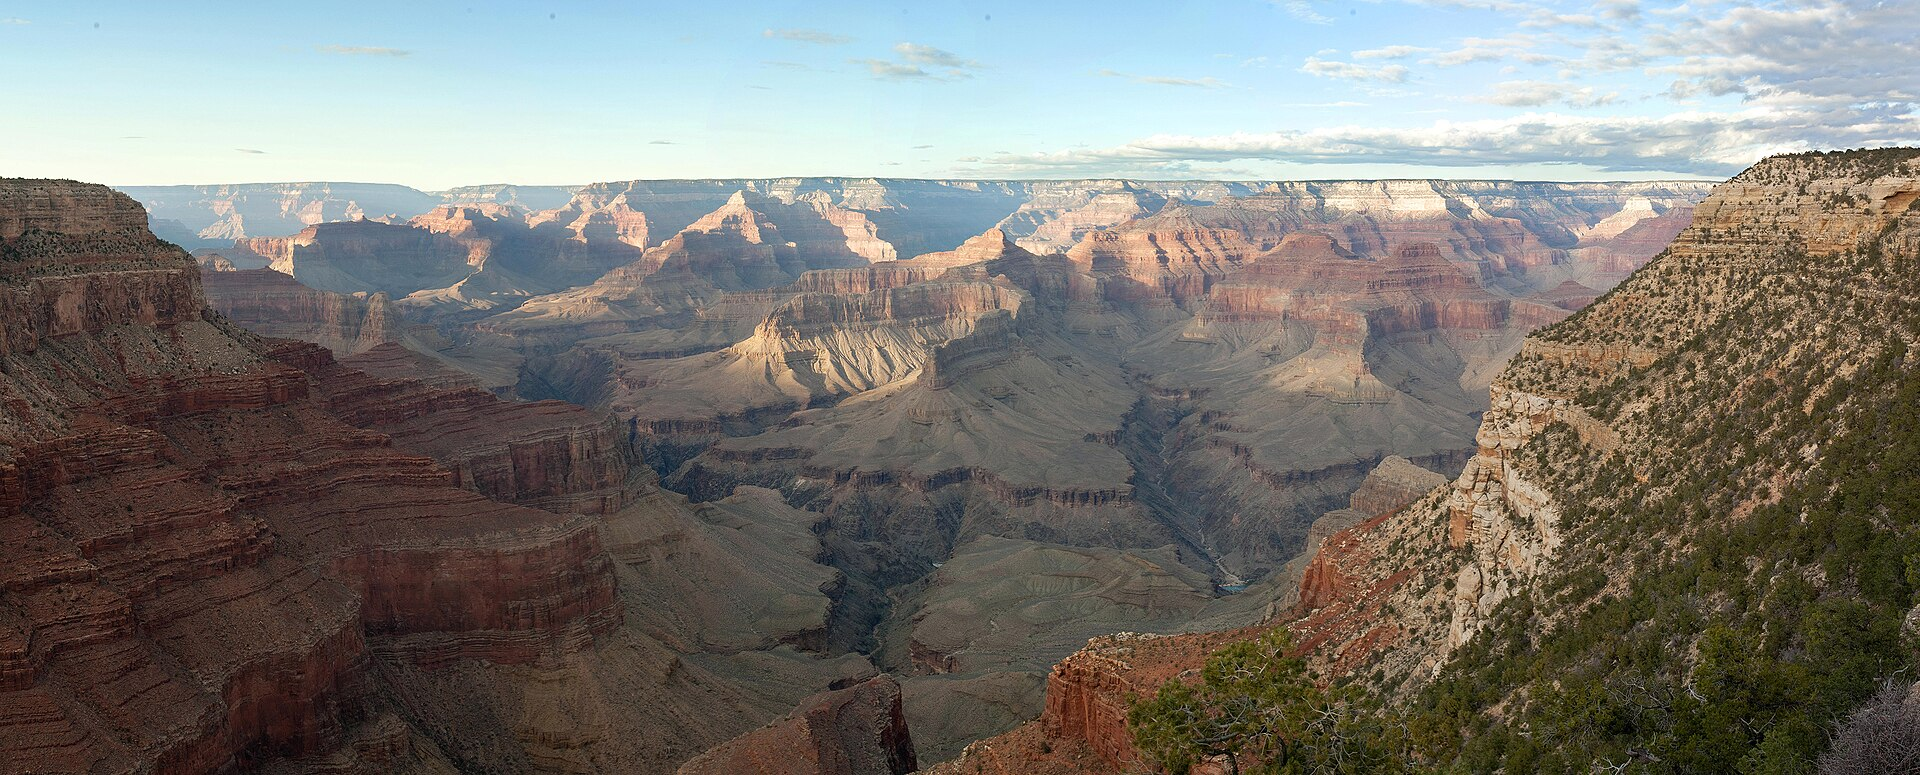
\includegraphics[width=\linewidth]{images/book1/g7-grand-canyon.jpg}

{\small الغراند كانيون من هيرميتس ريست، على حافته الجنوبية: طبقة بعد
طبقة من \omterm{def:g3:stones-pebbles-sand:rock}{الصخر}، من الحافة إلى القاع. صورة دائرة المتنزهات الوطنية
الأمريكية التقطتها كريستن~م. كالدون (ملك عام، عبر ويكيميديا كومنز).}
% ledger: commons:grand-canyon
\label{fig:g7:sediments-and-fossils:canyon}
\end{omfigure}

كيف تصير كومة من \omterm{def:g3:stones-pebbles-sand:sand}{الرمل} \omterm{def:g3:stones-pebbles-sand:sand}{والوحل} المفككين \omterm{def:g3:stones-pebbles-sand:rock}{صخرًا} صلبًا؟ وكيف يمكن لصدفة أن
تدوم زمنًا طويلًا حتى ينتهي بها المطاف داخل جرف؟ وماذا تخبرنا الطبقات
\omterm{def:g7:sediments-and-fossils:fossil}{والأحافير} عن الأماكن كما كانت منذ زمن بعيد؟

\begin{recall}
تتكسر \omterm{def:g3:stones-pebbles-sand:rock}{الصخور} ببطء إلى قطع على السطح (\emph{\omterm{def:g5:water-shapes-the-land:weathering}{التجوية}})؛ ويحمل الماء والريح
والجليد القطع بعيدًا (\emph{\omterm{def:g5:water-shapes-the-land:erosion}{التعرية}}) ويضعها حيث تتباطأ وتتوقف
(\emph{\omterm{def:g5:water-shapes-the-land:deposition}{الترسيب}}): الأثقل أولًا، \omterm{def:g3:stones-pebbles-sand:sand}{والوحل} الدقيق حيث يكاد الماء يسكن فقط
(\cref{ch:g5:water-shapes-the-land}). و\emph{\omterm{def:g6:rocks-and-minerals:rock-families}{الصخر الرسوبي}} يتكون على
السطح من حبيبات \omterm{def:g3:stones-pebbles-sand:sand}{الرمل} \omterm{def:g3:stones-pebbles-sand:sand}{والوحل}، أو من الأصداف، التي تترسب في طبقات ثم
تتصلب: الحجر الرملي، والسجّيل، والحجر الجيري. \omterm{def:g6:rocks-and-minerals:rock-cycle}{ودورة الصخور} تحوّل \omterm{def:g3:stones-pebbles-sand:rock}{صخور}
كل عائلة، ببطء، إلى \omterm{def:g3:stones-pebbles-sand:rock}{صخور} العائلتين الأخريين
(\cref{ch:g6:rocks-and-minerals}).
\end{recall}

\section{الرواسب تترسب في طبقات}

حيثما ألقى الماء أو الريح أو الجليد ما كان يحمله، تتراكم \omterm{def:g7:sediments-and-fossils:sediment}{رواسب} مفككة:
\omterm{def:g3:stones-pebbles-sand:pebble}{حصباء} \omterm{def:g3:stones-pebbles-sand:sand}{ورمل} في قاع \omterm{def:g1:landscapes-around-us:water}{نهر}، \omterm{def:g3:stones-pebbles-sand:sand}{ووحل} في قاع \omterm{def:g1:landscapes-around-us:water}{بحيرة}، \omterm{def:g3:stones-pebbles-sand:sand}{ورمل} على شاطئ أو في كثيب،
وأصداف في قاع \omterm{def:g2:water-on-earth:ocean}{البحر}.

\begin{definition}[الرواسب]\label{def:g7:sediments-and-fossils:sediment}
\emph{الرواسب}\index{رواسب} مواد مفككة يضعها الماء أو الريح أو الجليد:
\omterm{def:g3:stones-pebbles-sand:pebble}{حصباء}، \omterm{def:g3:stones-pebbles-sand:sand}{ورمل}، \omterm{def:g3:stones-pebbles-sand:sand}{ووحل}، أو أصداف الكائنات الحية وهياكلها. وهي تتجمع في قيعان
\omterm{def:g1:landscapes-around-us:water}{الأنهار} \omterm{def:g1:landscapes-around-us:water}{والبحيرات} والبحار، وعلى اليابسة حيث تلقيها الريح أو الجليد.
\end{definition}

تترسب \omterm{def:g7:sediments-and-fossils:sediment}{الرواسب} بترتيب معين. فحين يتباطأ ماء موحل، تغوص أكبر الحبيبات
وأثقلها أولًا، وأصغرها وأخفها أخيرًا. وكلما تغير الماء --- \omterm{def:g5:water-shapes-the-land:flood}{فيضان} يجلب
\omterm{def:g3:stones-pebbles-sand:sand}{الرمل}، ثم أسابيع هادئة لا يبلغ فيها القاع إلا \omterm{def:g3:stones-pebbles-sand:sand}{الوحل} الدقيق --- تغيرت
الحبيبات التي تترسب أيضًا، وبدأت طبقة جديدة. وشيئًا فشيئًا، يُغطى قاع
\omterm{def:g1:landscapes-around-us:water}{البحيرة} أو \omterm{def:g2:water-on-earth:ocean}{البحر} بكومة من الطبقات، أقدمها في أسفل الكومة.
% ledger: usgs:strata, usgs:sediments-to-rock

\begin{omfigure}
\begin{tikzpicture}[font=\small, x=1cm, y=1cm]
  % land and river
  \fill[omLithAlluv] (0,3.0) -- (2.0,2.45) -- (2.0,0) -- (0,0) -- cycle;
  \fill[blue!35] (0,3.05) -- (2.0,2.5) -- (2.0,2.4) -- (0,2.95) -- cycle;
  % lake water
  \fill[omSea!45] (2.0,2.5) -- (12.4,2.5) -- (12.4,1.12) -- (3.0,1.2) -- cycle;
  \draw[blue!50!black, line width=0.6pt] (2.0,2.5) -- (12.4,2.5);
  % layers on the bottom: thick near the mouth, thinner far out
  \foreach \k/\c in {0/omLithSand, 1/omLithShale, 2/omLithSand, 3/omLithShale} {
    \pgfmathsetmacro{\yb}{0.2+0.25*\k}
    \pgfmathsetmacro{\yt}{0.2+0.25*(\k+1)}
    \fill[\c] (3.0,\yb) -- (12.4,\yb) -- (12.4,\yt-0.08) -- (3.0,\yt) -- cycle;
  }
  \draw[black!60, line width=0.3pt] (3.0,1.2) -- (12.4,1.12);
  \fill[omLithAlluv!80!black] (2.0,0) rectangle (12.4,0.2);
  \fill[omLithAlluv] (2.0,0.2) -- (3.0,0.2) -- (3.0,1.2) -- (2.0,2.45) -- cycle;
  % settling grains: big ones near the mouth, fine ones far out
  \foreach \x/\y in {3.3/2.1, 3.6/1.75, 3.9/2.25, 4.2/1.55, 3.5/1.35, 4.5/2.0} {
    \fill[brown!70!black] (\x,\y) circle (0.07);
    \draw[-{Stealth[length=1.3mm]}, black!60] (\x,\y-0.1) -- (\x,\y-0.32);
  }
  \foreach \x/\y in {6.5/2.2, 7.4/1.8, 8.3/2.15, 9.1/1.6, 9.9/2.05, 10.8/1.75, 11.6/2.1, 7.9/1.35, 10.4/1.3} {
    \fill[brown!50!black] (\x,\y) circle (0.025);
    \draw[-{Stealth[length=1mm]}, black!40] (\x,\y-0.05) -- (\x,\y-0.2);
  }
  \node[anchor=south, align=center] at (1.0,3.1) {نهر في فيضان\\[-2pt]يجلب الرمل والوحل};
  \node[anchor=south, align=center] at (4.1,2.55) {يترسب الرمل أولًا\\[-2pt]قرب المصب};
  \node[anchor=south, align=center] at (9.2,2.55) {يترسب الوحل الدقيق ببطء\\[-2pt]بعيدًا حيث الماء هادئ};
  \draw[decorate, decoration={brace, amplitude=4pt}] (12.55,1.15) -- (12.55,0.2)
    node[midway, anchor=west, xshift=4pt, align=left, font=\footnotesize] {طبقات في القاع\\[-2pt]رمل ثم وحل\\[-2pt]ثم رمل ثم وحل};
\end{tikzpicture}

{\small \omterm{def:g7:sediments-and-fossils:sediment}{رواسب} تترسب في \omterm{def:g1:landscapes-around-us:water}{بحيرة} (رسم، ليس بمقياس رسم). بعد كل \omterm{def:g5:water-shapes-the-land:flood}{فيضان} تترسب
طبقة من \omterm{def:g3:stones-pebbles-sand:sand}{الرمل}، ثم \omterm{def:g3:stones-pebbles-sand:sand}{الوحل} الدقيق في الأسابيع الهادئة التي تليه: وهكذا
تتراكم طبقة بعد طبقة في القاع.}
% ledger: usgs:strata
\label{fig:g7:sediments-and-fossils:lake}
\end{omfigure}

\begin{definition}[الطبقة الرسوبية]\label{def:g7:sediments-and-fossils:layer}
\emph{الطبقة الرسوبية}\index{طبقة رسوبية}، أو \emph{الطبقة
الصخرية}\index{طبقة صخرية} (وجمعها \emph{طبقات صخرية})، صفيحة من \omterm{def:g7:sediments-and-fossils:sediment}{الرواسب}،
أو من \omterm{def:g3:stones-pebbles-sand:rock}{الصخر} الذي صارت إليه، وُضعت في وقت واحد. ولها قاعدة وسطح، وهي
تختلف عن الطبقتين اللتين فوقها وتحتها في حجم حبيباتها أو في المادة
التي تتكون منها.
\end{definition}

تترسب \omterm{def:g7:sediments-and-fossils:sediment}{الرواسب} من الماء أو الهواء، ولذلك توضع مستوية، كصفحات كتاب ملقى
على طاولة. وحين نجد طبقات مائلة أو مطوية، فذلك لأن شيئًا حرّكها بعد أن
تكونت. والتطبق أوضح علامات \omterm{def:g6:rocks-and-minerals:rock-families}{الصخر الرسوبي}: وقد رأيته في جدران الغراند
كانيون.
% ledger: usgs:strata, nps:grca-kaibab

\begin{inthelab}[طبقات في وعاء زجاجي (في القسم، مع المعلم)]
ضع حفنة من \omterm{def:g3:stones-pebbles-sand:pebble}{الحصباء}، وحفنتين من \omterm{def:g3:stones-pebbles-sand:sand}{الرمل}، وبضع ملاعق من التراب في وعاء زجاجي
طويل؛ واملأه بالماء، وأغلقه بإحكام ثم رجّه. ضعه وراقبه بضع دقائق: تبلغ
\omterm{def:g3:stones-pebbles-sand:pebble}{الحصباء} القاع على الفور، \omterm{def:g3:stones-pebbles-sand:sand}{والرمل} بعدها بقليل، ويبقي \omterm{def:g3:stones-pebbles-sand:sand}{الوحل} الدقيق الماء
عكرًا ساعات. وفي اليوم التالي، أضف قليلًا من التراب \omterm{def:g3:stones-pebbles-sand:sand}{والرمل}، ورجّه برفق،
واتركه يترسب من جديد. كم طبقة تستطيع أن تعدّ؟ وأي الحبيبات في أسفل كل
طبقة منها؟
\end{inthelab}

\section{من الرواسب إلى الصخر}

لا تبقى الطبقة في الأعلى زمنًا طويلًا. فطبقات أخرى تترسب فوقها، ثم
غيرها، فتُدفن أعمق فأعمق. وتحت ثقل الطبقات التي فوقها، تنضغط الحبيبات
بعضها إلى بعض ويُعصر الماء الذي بينها إلى الخارج. والماء المتسرب عبر
الكومة يترك بين الحبيبات \omterm{def:g6:rocks-and-minerals:mineral}{معادن}، هي إسمنت طبيعي يلصقها بعضها ببعض. ومع
مرور زمن طويل، وتراكم مزيد من الطبقات، وتغيرات كيميائية بطيئة، تصير
\omterm{def:g7:sediments-and-fossils:sediment}{الرواسب} المفككة في أسفل الكومة \omterm{def:g3:stones-pebbles-sand:rock}{صخرًا}.
% ledger: usgs:sediments-to-rock, usgs:sedimentary

ولكل نوع من \omterm{def:g7:sediments-and-fossils:sediment}{الرواسب} صخره الخاص.

\begin{center}
\small
\begin{tabular}{|l|l|}
\hline
\textbf{\omterm{def:g7:sediments-and-fossils:sediment}{الرواسب}} & \textbf{\omterm{def:g3:stones-pebbles-sand:rock}{الصخر} الذي تصير إليه} \\
\hline
\omterm{def:g3:stones-pebbles-sand:pebble}{الحصباء} \omterm{def:g3:stones-pebbles-sand:pebble}{والحصى} & الرصيص \\
\omterm{def:g3:stones-pebbles-sand:sand}{الرمل} & الحجر الرملي \\
\omterm{def:g3:stones-pebbles-sand:sand}{الوحل} & الحجر الطيني، أو السجّيل حين ينفلق إلى صفائح رقيقة \\
الأصداف والهياكل & الحجر الجيري \\
بقايا النباتات، مدفونة في مستنقع & الفحم \\
\hline
\end{tabular}
\end{center}
% ledger: usgs:sediments-to-rock, usgs:sedimentary, usgs:coal-origin

\begin{omfigure}
\begin{tikzpicture}[font=\small, x=1cm, y=1cm]
  \pgfmathsetseed{11}
  \foreach \p/\gap/\title in {0/0.40/{رواسب مفككة}, 1/0.31/{مدفونة ومضغوطة\\[-2pt]يُطرد منها الماء}, 2/0.31/{ملتحمة فصارت صخرًا}} {
    \begin{scope}[xshift=\p*4.6cm]
      \ifnum\p=2 \fill[black!25] (0,0) rectangle (3.4,3.0);
      \else \fill[omSea!45] (0,0) rectangle (3.4,3.0); \fi
      \foreach \i in {0,...,7} {
        \foreach \j in {0,...,6} {
          \pgfmathsetmacro{\gx}{0.25 + \i*\gap*1.05 + 0.05*rand}
          \pgfmathsetmacro{\gy}{0.25 + \j*\gap + 0.05*rand}
          \pgfmathsetmacro{\gr}{0.13 + 0.03*rand}
          \ifdim\gx pt<3.25pt \ifdim\gy pt<2.85pt
            \fill[omLithSand!80!brown, draw=brown!60!black, line width=0.3pt] (\gx,\gy) circle (\gr);
          \fi\fi
        }
      }
      \draw[black!70, line width=0.6pt] (0,0) rectangle (3.4,3.0);
      \node[anchor=north, align=center] at (1.7,-0.1) {\title};
    \end{scope}
  }
  \draw[-{Stealth[length=2.5mm]}, line width=1pt] (3.6,1.5) -- (4.4,1.5);
  \draw[-{Stealth[length=2.5mm]}, line width=1pt] (8.2,1.5) -- (9.0,1.5);
  \foreach \x in {5.3,6.3,7.3} \draw[-{Stealth[length=2mm]}, line width=0.8pt] (\x,3.7) -- (\x,3.1);
  \node[anchor=south] at (6.3,3.7) {ثقل الطبقات التي فوقها};
  \node[anchor=south, font=\footnotesize, align=center] at (10.9,3.05) {بالرمادي: الإسمنت الطبيعي};
\end{tikzpicture}

{\small من \omterm{def:g3:stones-pebbles-sand:sand}{الرمل} إلى الحجر الرملي (رسم للحبيبات، مكبَّر كثيرًا). على
اليسار: حبيبات مفككة بينها ماء. في الوسط: مدفونة تحت طبقات جديدة، فتنضغط
الحبيبات بعضها إلى بعض. على اليمين: \omterm{def:g6:rocks-and-minerals:mineral}{المعادن} التي تركها الماء تلصق
الحبيبات بعضها ببعض.}
% ledger: usgs:sediments-to-rock, usgs:sedimentary
\label{fig:g7:sediments-and-fossils:to-rock}
\end{omfigure}

معظم \omterm{def:g3:stones-pebbles-sand:rock}{الصخور} التي تستطيع أن تراها على سطح الأرض \omterm{def:g6:rocks-and-minerals:rock-families}{صخور رسوبية}. وكومة الطبقات
التي تشكّلها هي كتاب تاريخ المكان: كل طبقة صفحة، وأقدم الصفحات في
الأسفل.
% ledger: usgs:sediments-to-rock

\section{كيف تتكون الأحفورة}

\begin{definition}[الأحفورة]\label{def:g7:sediments-and-fossils:fossil}
\emph{الأحفورة}\index{أحفورة} بقايا كائن حي من زمن بعيد، أو أثره، محفوظة
في \omterm{def:g3:stones-pebbles-sand:rock}{الصخر}. فبعض الأحافير أجزاء صلبة من الجسم --- صدفة، أو عظم، أو سن، أو
خشب --- تحولت إلى حجر. وبعضها لا يحفظ إلا شكلًا: \emph{القالب}\index{قالب}
هو الطبعة المجوفة التي تبقى في \omterm{def:g3:stones-pebbles-sand:rock}{الصخر} حيث ذابت صدفة أو عظم؛
و\emph{المصبوبة}\index{مصبوبة} هي النسخة التي تتكون حين يمتلئ القالب بمادة
معدنية جديدة أو \omterm{def:g7:sediments-and-fossils:sediment}{برواسب}. و\emph{الأحفورة الأثرية}\index{أحفورة أثرية}
علامة على ما فعله حيوان --- أثر قدم، أو جحر، أو مسار --- وليست جزءًا
من جسمه.
\end{definition}

تبدأ \omterm{def:g7:sediments-and-fossils:fossil}{الأحفورة} حياتها حيوانًا أو نباتًا ميتًا في قاع \omterm{def:g2:water-on-earth:ocean}{بحر} أو \omterm{def:g1:landscapes-around-us:water}{بحيرة}. فإن
بقي مكشوفًا، حللته البكتيريا وأذاب الماء ببطء ما يبقى منه. ولا تكون له
فرصة إلا إذا دُفن بسرعة، تحت \omterm{def:g7:sediments-and-fossils:sediment}{رواسب} تترسب فوقه وتعزله. ثم، بينما تتحول
\omterm{def:g7:sediments-and-fossils:sediment}{الرواسب} إلى \omterm{def:g3:stones-pebbles-sand:rock}{صخر}، يجلب الماء المتسرب عبر الطبقات \omterm{def:g6:rocks-and-minerals:mineral}{معادن} تملأ كل ثقب دقيق
في الصدفة أو العظم: فيتحول إلى حجر. وبعد ذلك بزمن طويل، قد تتآكل
الطبقات التي فوقه، فتظهر \omterm{def:g7:sediments-and-fossils:fossil}{الأحفورة} على السطح.
% ledger: ucmp:fossil-conditions, ucmp:fossil-kinds, usgs:sediments-to-rock

\begin{omfigure}
\begin{tikzpicture}[font=\small, x=0.86cm, y=0.86cm,
    shell/.pic={
      \fill[#1] (0,0) circle (0.42);
      \draw[brown!40!black, line width=0.5pt] plot[domain=0:12.5, samples=90, smooth]
        ({0.032*\x*cos(\x r)}, {0.032*\x*sin(\x r)});
      \draw[brown!40!black, line width=0.5pt] (0,0) circle (0.42);
    }]
  % 1: death on the sea floor
  \begin{scope}[xshift=0cm]
    \fill[omSea!45] (0,1.2) rectangle (3.3,3.6);
    \fill[omLithShale] (0,0) rectangle (3.3,1.2);
    \pic at (1.65,1.62) {shell=omLithSand!60!white};
    \node[anchor=north, align=center] at (1.65,-0.1) {\foreignlanguage{arabic}{1. يموت في}\\[-2pt]قاع البحر};
  \end{scope}
  % 2: quick burial
  \begin{scope}[xshift=3.75cm]
    \fill[omSea!45] (0,2.1) rectangle (3.3,3.6);
    \fill[omLithShale] (0,0) rectangle (3.3,1.2);
    \fill[omLithShale!70!white] (0,1.2) rectangle (3.3,2.1);
    \pic at (1.65,1.62) {shell=omLithSand!60!white};
    \foreach \x in {0.5,1.2,2.1,2.8} \fill[brown!50!black] (\x,2.4) circle (0.03);
    \node[anchor=north, align=center] at (1.65,-0.1) {\foreignlanguage{arabic}{2. يغطيه الوحل}\\[-2pt]بسرعة};
  \end{scope}
  % 3: buried deep, turned to stone
  \begin{scope}[xshift=7.5cm]
    \fill[omLithShale!80!black] (0,0) rectangle (3.3,1.2);
    \fill[omLithShale!85!black] (0,1.2) rectangle (3.3,2.1);
    \fill[omLithSand] (0,2.1) rectangle (3.3,2.9);
    \fill[omLithLime] (0,2.9) rectangle (3.3,3.6);
    \pic at (1.65,1.62) {shell=black!35};
    \node[anchor=north, align=center] at (1.65,-0.1) {\foreignlanguage{arabic}{3. مدفونًا في العمق}\\[-2pt]يتحول إلى حجر};
  \end{scope}
  % 4: uncovered by erosion
  \begin{scope}[xshift=11.25cm]
    \fill[white] (0,0) rectangle (3.3,3.6);
    \fill[omLithShale!80!black] (0,0) -- (3.3,0) -- (3.3,2.6) -- (2.4,2.3) -- (1.8,1.95) -- (1.2,1.7) -- (0,1.5) -- cycle;
    \draw[black!35, line width=0.4pt] (0,1.2) -- (3.3,1.2);
    \draw[black!60, line width=0.4pt] (0,1.5) -- (1.2,1.7) -- (1.8,1.95) -- (2.4,2.3) -- (3.3,2.6);
    \pic at (1.65,1.84) {shell=black!35};
    \node[anchor=north, align=center] at (1.65,-0.1) {\foreignlanguage{arabic}{4. التعرية}\\[-2pt]تعيده إلى السطح};
  \end{scope}
  \foreach \p in {0,1,2,3} {
    \begin{scope}[xshift=\p*3.75cm]
      \draw[black!70, line width=0.5pt] (0,0) rectangle (3.3,3.6);
    \end{scope}
  }
\end{tikzpicture}

{\small كيف تتكون \omterm{def:g7:sediments-and-fossils:fossil}{الأحفورة} (رسم، ليس بمقياس رسم): تُدفن صدفة بسرعة تحت
\omterm{def:g3:stones-pebbles-sand:sand}{الوحل}؛ ثم تُدفن أعمق تحت طبقات جديدة فتتحول إلى حجر؛ وبعد ذلك بزمن طويل،
تبري \omterm{def:g5:water-shapes-the-land:erosion}{التعرية} الطبقات التي فوقها فتظهر \omterm{def:g7:sediments-and-fossils:fossil}{الأحفورة} على السطح.}
% ledger: ucmp:fossil-conditions, ucmp:fossil-kinds
\label{fig:g7:sediments-and-fossils:steps}
\end{omfigure}

معظم الكائنات الحية لا تترك أي \omterm{def:g7:sediments-and-fossils:fossil}{أحفورة}. فالأجسام الطرية تتعفن قبل أن
تُدفن؛ وحتى الأصداف والعظام تنكسر أو تذوب إذا بقيت مكشوفة زمنًا طويلًا.
وأفضل مكان لتصير الكائنات \omterm{def:g7:sediments-and-fossils:fossil}{أحافير} هو قاع \omterm{def:g2:water-on-earth:ocean}{بحر} أو \omterm{def:g1:landscapes-around-us:water}{بحيرة} هادئين، حيث يترسب
\omterm{def:g3:stones-pebbles-sand:sand}{الوحل} الدقيق فوق البقايا ويحميها. ولهذا فإن \omterm{def:g7:sediments-and-fossils:fossil}{الأحافير} التي توجد في
\omterm{def:g3:stones-pebbles-sand:rock}{الصخور} هي في معظمها أصداف، وأصداف دقيقة وبقايا نباتات وحيوانات مجهرية؛
أما الديناصورات، أشهر \omterm{def:g7:sediments-and-fossils:fossil}{الأحافير}، فليست إلا جزءًا صغيرًا جدًا منها.
% ledger: ucmp:fossil-conditions, usgs:fossil-record-shells

\begin{omfigure}
\begin{minipage}[t]{0.49\linewidth}\centering
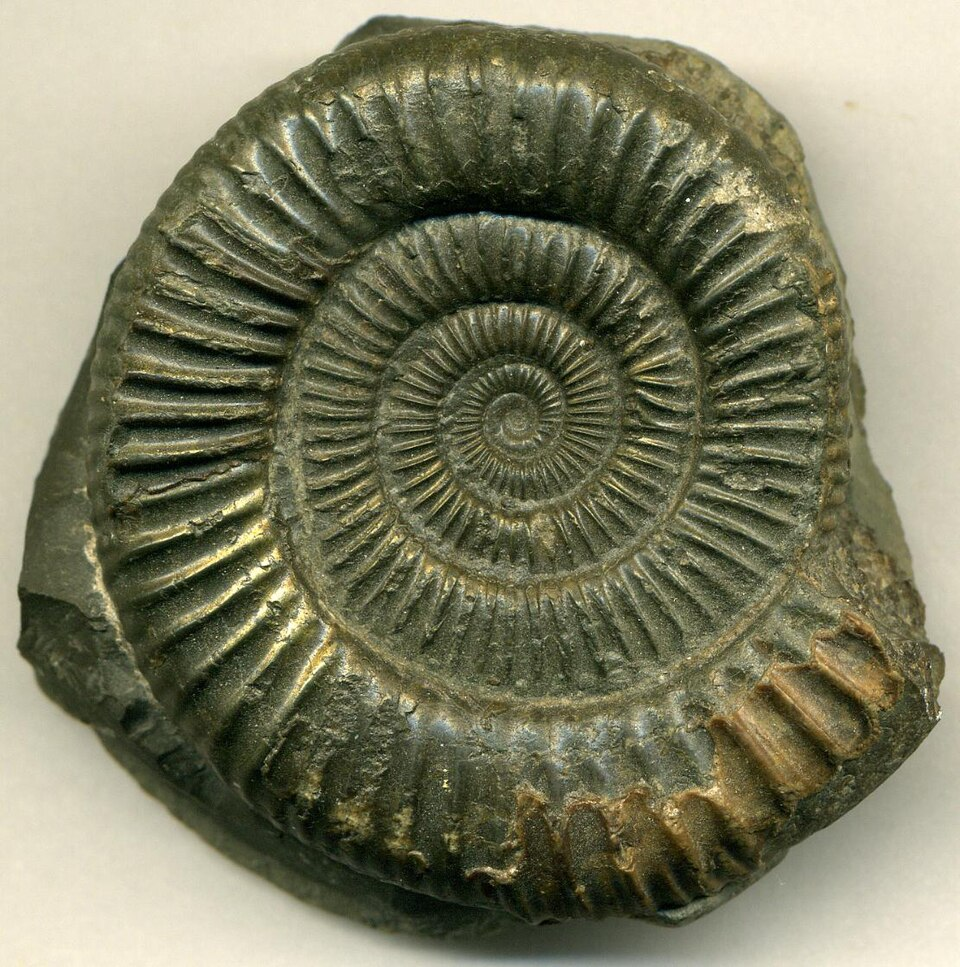
\includegraphics[height=4.6cm]{images/book1/g7-ammonite.jpg}

{\small أمونيت، حيوان منقرض ذو صدفة ملتفة، من أقارب الحبّار
والأخطبوط، عرضه \qty{5.7}{cm}، من \omterm{def:g1:landscapes-around-us:water}{ساحل} يوركشاير
(إنجلترا).}
\end{minipage}\hfill
\begin{minipage}[t]{0.49\linewidth}\centering
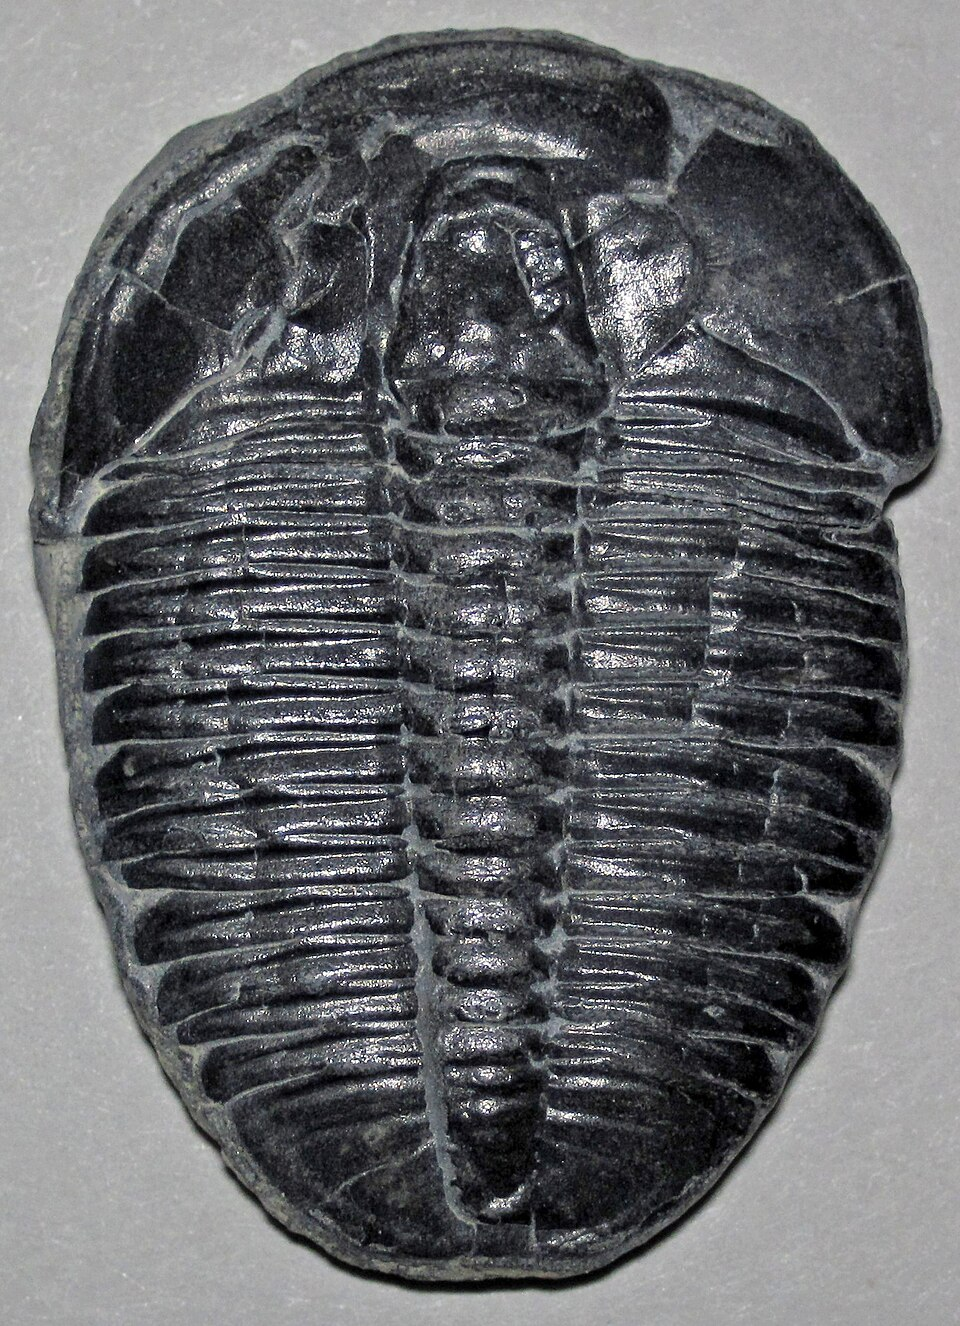
\includegraphics[height=4.6cm]{images/book1/g7-trilobite.jpg}

{\small ثلاثي فصوص، حيوان بحري منقرض جسمه ثلاثة فصوص، عرضه نحو
\qty{2.6}{cm}، من يوتا (الولايات المتحدة).}
\end{minipage}\par\medskip

{\small أحفورتان لحيوانين ذوي أصداف صلبة. الصورتان: جيمس
سانت~جون (CC BY 2.0، عبر ويكيميديا كومنز).}
% ledger: commons:ammonite, commons:trilobite, nps:ammonoid, nps:trilobite
\label{fig:g7:sediments-and-fossils:ammonite-trilobite}
\end{omfigure}

أحيانًا لا تدوم الصدفة نفسها. فإذا دُفنت في \omterm{def:g3:stones-pebbles-sand:sand}{الرمل}، أذابها ببطء الماء
المتسرب بين الحبيبات، ولا يبقى إلا تجويف، شكل الصدفة مطبوع على جدرانه:
إنه \omterm{def:g7:sediments-and-fossils:fossil}{القالب}. فإذا ترسبت فيه \omterm{def:g6:rocks-and-minerals:mineral}{معادن} لاحقًا وملأته، صنعت نسخة من الصدفة:
إنها \omterm{def:g7:sediments-and-fossils:fossil}{المصبوبة}.
% ledger: ucmp:casts-molds

\begin{omfigure}
\begin{tikzpicture}[font=\small, x=1cm, y=1cm,
    clam/.style={line width=0.5pt}]
  \foreach \p/\fillc/\title in {0/{omLithSand!50!white}/{صدفة مدفونة\\[-2pt]في الرمل}, 1/{white}/{ذابت الصدفة\\[-2pt]فبقي قالب}, 2/{black!40}/{معادن تملأ القالب\\[-2pt]فتتكون مصبوبة}} {
    \begin{scope}[xshift=\p*4.9cm]
      \fill[omLithSand] (0,0) rectangle (4.2,2.6);
      \foreach \i in {0,...,40} {
        \pgfmathsetmacro{\gx}{0.1+mod(\i*0.53,4.0)}
        \pgfmathsetmacro{\gy}{0.1+mod(\i*0.37,2.4)}
        \fill[brown!60!black] (\gx,\gy) circle (0.025);
      }
      \fill[\fillc, draw=brown!40!black, clam] (0.9,0.9) arc[start angle=180, end angle=0, x radius=1.2, y radius=0.95] -- cycle;
      \ifnum\p=1
        \foreach \a in {25,45,...,155} \draw[brown!50!black, line width=0.4pt] (2.1,0.9) -- ++(\a:0.93 and 0.75);
      \else
        \foreach \a in {25,45,...,155} \draw[brown!40!black, line width=0.4pt] (2.1,0.9) -- ++(\a:1.05 and 0.85);
      \fi
      \draw[black!70, line width=0.5pt] (0,0) rectangle (4.2,2.6);
      \node[anchor=north, align=center] at (2.1,-0.1) {\title};
    \end{scope}
  }
  \draw[-{Stealth[length=2.5mm]}, line width=1pt] (4.3,1.3) -- (4.8,1.3);
  \draw[-{Stealth[length=2.5mm]}, line width=1pt] (9.2,1.3) -- (9.7,1.3);
\end{tikzpicture}

{\small \omterm{def:g7:sediments-and-fossils:fossil}{قالب} \omterm{def:g7:sediments-and-fossils:fossil}{ومصبوبة} (رسم، مقطع في \omterm{def:g3:stones-pebbles-sand:rock}{الصخر}). \omterm{def:g7:sediments-and-fossils:fossil}{القالب} هو التجويف، وأضلاع
الصدفة مطبوعة على جداره؛ \omterm{def:g7:sediments-and-fossils:fossil}{والمصبوبة} نسخة حجرية من الصدفة، مصنوعة من
\omterm{def:g6:rocks-and-minerals:mineral}{المعادن} التي ملأته.}
% ledger: ucmp:casts-molds
\label{fig:g7:sediments-and-fossils:mould-cast}
\end{omfigure}

تترك الحيوانات أيضًا \omterm{def:g7:sediments-and-fossils:fossil}{أحافير} لما فعلته. فالحيوان الذي يمشي على \omterm{def:g3:stones-pebbles-sand:sand}{الوحل}
الطري المبلل لضفة \omterm{def:g1:landscapes-around-us:water}{نهر} أو لشاطئ يترك آثار أقدام. ومعظمها تمحوه الموجة
التالية أو \omterm{def:g5:water-shapes-the-land:flood}{الفيضان} التالي. لكن إذا غطاها \omterm{def:g3:stones-pebbles-sand:sand}{الرمل} قبل أن تُمحى، امتلأ
أثر القدم، ثم صار \omterm{def:g3:stones-pebbles-sand:sand}{الرمل} حجرًا رمليًا، وحين ينفلق \omterm{def:g3:stones-pebbles-sand:rock}{الصخر} على طول الطبقة،
يظهر أثر القدم، وعلى الوجه الآخر مصبوبته.
% ledger: ucmp:footprints

\begin{omfigure}
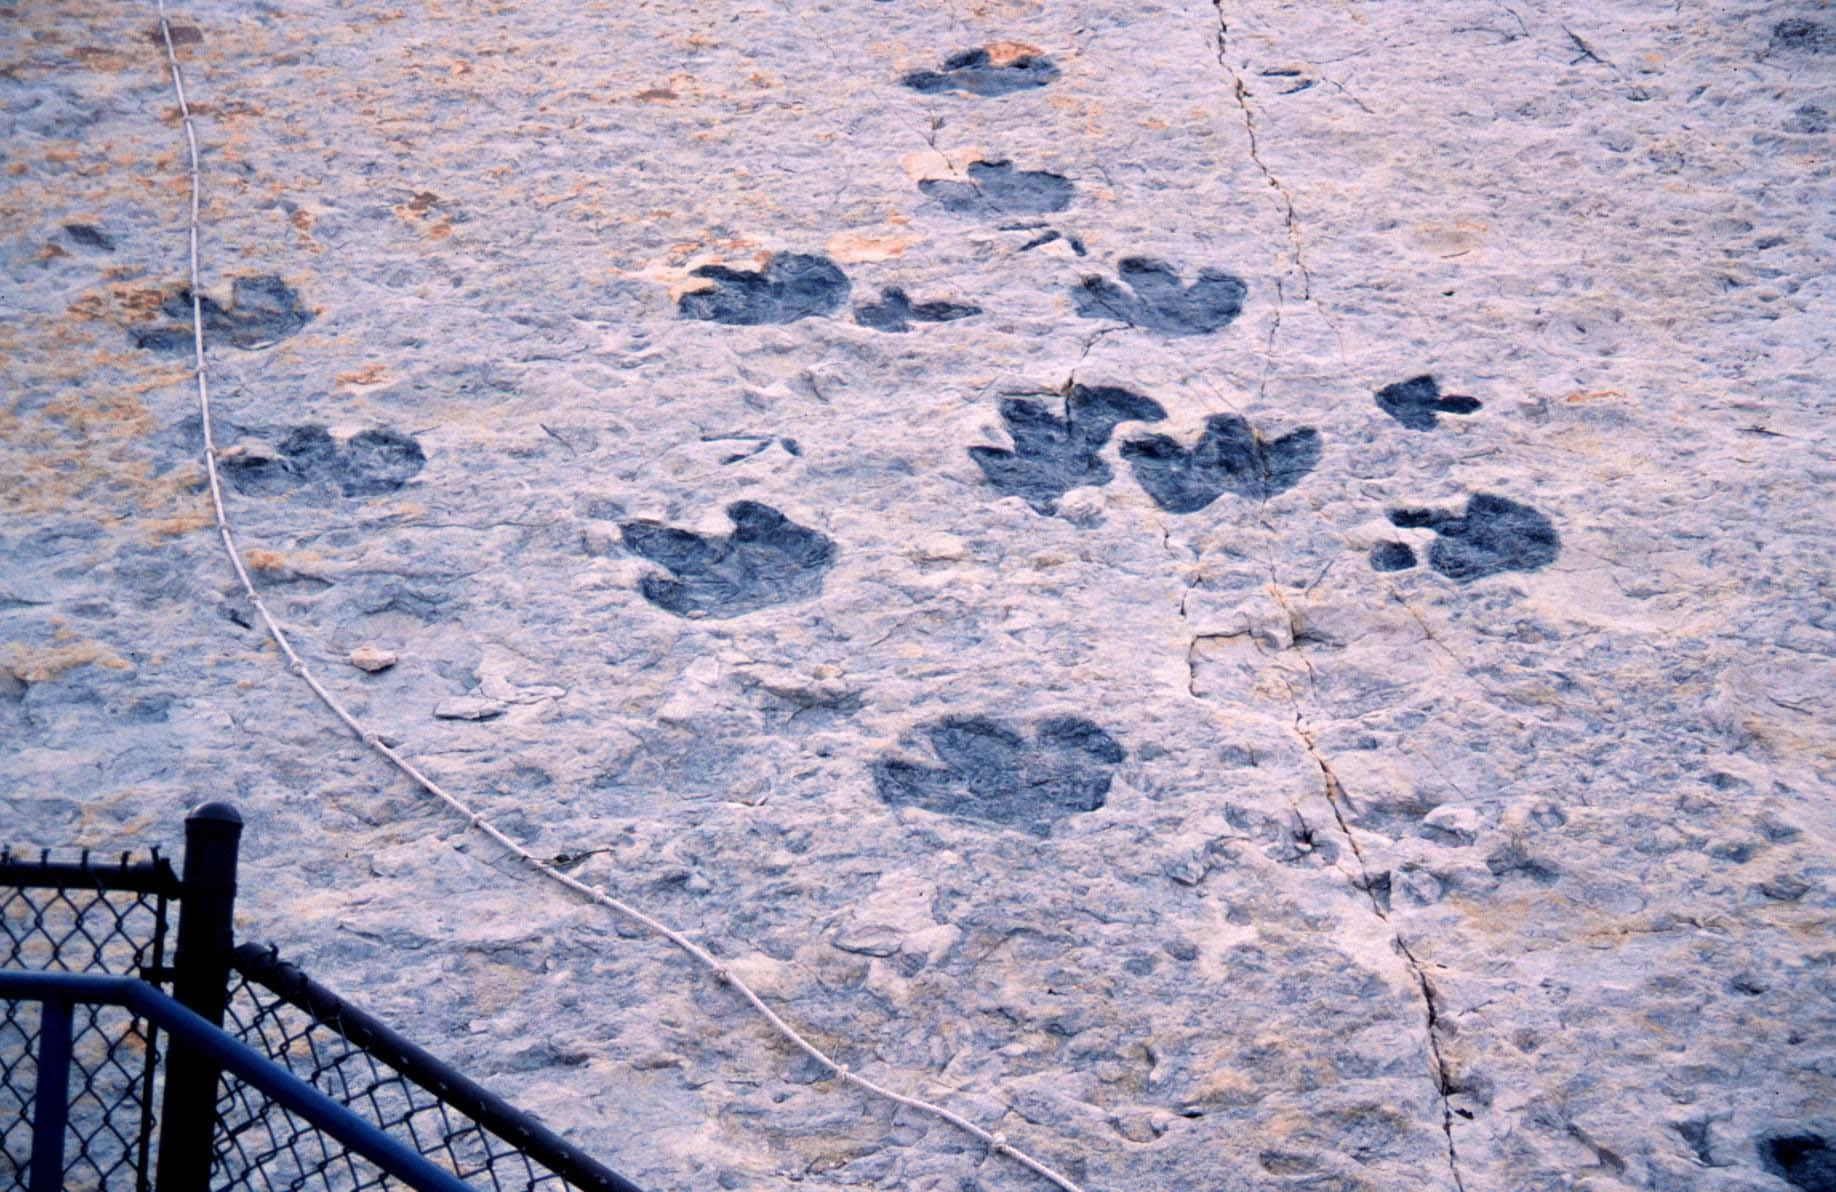
\includegraphics[width=0.62\linewidth]{images/book1/g7-dinosaur-tracks.jpg}

{\small آثار أقدام ديناصورات في دايناسور ريدج، قرب موريسون، في كولورادو
(الولايات المتحدة): عشرات الآثار تُركت في أرض طرية، وهي اليوم سطح صخري
مائل. ومعظمها تركته ديناصورات آكلة للنبات، وبعضها القليل تركته ديناصورات
آكلة للحوم ذات أصابع نحيلة. الصورة: دكستر بيركنز (CC0، عبر ويكيميديا
كومنز).}
% ledger: commons:dino-tracks
\label{fig:g7:sediments-and-fossils:tracks}
\end{omfigure}

يستعمل علم الأحياء \omterm{def:g7:sediments-and-fossils:fossil}{الأحافير} لتتبع التاريخ الطويل للكائنات الحية. أما في
هذا الكتاب، \omterm{def:g7:sediments-and-fossils:fossil}{فالأحافير} أدلة من نوع آخر: إنها تخبرنا كيف كان المكان حين
عاش فيه الحيوان.

\section{الطبقات والأحافير، سجل للماضي}

تحفظ كل طبقة علامات المكان الذي وُضعت فيه. فالشعاب المرجانية تنمو اليوم في
بحار دافئة صافية ضحلة؛ وعلامات التموج تتكون على \omterm{def:g3:stones-pebbles-sand:sand}{الرمل} في المياه الضحلة،
على حافة \omterm{def:g1:landscapes-around-us:water}{بحيرة} أو \omterm{def:g1:landscapes-around-us:water}{نهر} أو \omterm{def:g2:water-on-earth:ocean}{بحر}؛ والفحم تكوَّن من نباتات غابات ومستنقعات
قديمة؛ وعضديات الأرجل وزنبقيات \omterm{def:g2:water-on-earth:ocean}{البحر} وثلاثيات الفصوص لم تعش إلا في \omterm{def:g2:water-on-earth:ocean}{البحر}.
وحين نجد الأدلة نفسها في طبقة قديمة، فالأرجح أن المكان كان كذلك حين
تكونت الطبقة.
% ledger: noaa:coral-where, nps:ripple-marks, nps:ripples-shallow, usgs:coal-origin, nps:trilobite

\begin{center}
\small
\begin{tabular}{|p{0.36\linewidth}|p{0.52\linewidth}|}
\hline
\textbf{الدليل في الطبقة} & \textbf{المكان حين تكونت الطبقة} \\
\hline
المرجان & \omterm{def:g2:water-on-earth:ocean}{بحر} دافئ ضحل صافٍ \\
\hline
أصداف حيوانات بحرية (عضديات الأرجل، زنبقيات \omterm{def:g2:water-on-earth:ocean}{البحر}، ثلاثيات الفصوص) & \omterm{def:g2:water-on-earth:ocean}{بحر} \\
\hline
علامات تموج على سطح طبقة & مياه ضحلة، على حافة \omterm{def:g1:landscapes-around-us:water}{بحيرة} أو \omterm{def:g1:landscapes-around-us:water}{نهر} أو \omterm{def:g2:water-on-earth:ocean}{بحر} \\
\hline
آثار أقدام & \omterm{def:g3:stones-pebbles-sand:sand}{وحل} أو \omterm{def:g3:stones-pebbles-sand:sand}{رمل} طري مبلل، كثيرًا ما يكون على شاطئ أو ضفة \omterm{def:g1:landscapes-around-us:water}{نهر} \\
\hline
الفحم & غابة مستنقعية أو مستنقع \\
\hline
أوراق نبات وأجنحة يعاسيب & يابسة، تنمو عليها نباتات \\
\hline
\end{tabular}
\end{center}
% ledger: noaa:coral-where, nps:grca-fossils, nps:trilobite, nps:ripple-marks, nps:ripples-shallow, ucmp:footprints, usgs:coal-origin

\begin{method}[قراءة طبقة]\label{met:g7:sediments-and-fossils:reading}
\begin{enumerate}
  \item انظر إلى الحبيبات: الحبيبات الخشنة تترسب حيث يتحرك الماء بسرعة،
        \omterm{def:g3:stones-pebbles-sand:sand}{والوحل} الدقيق حيث يكون هادئًا فقط.
  \item ابحث عن \omterm{def:g7:sediments-and-fossils:fossil}{الأحافير} والعلامات (مرجان، أصداف، آثار أقدام، علامات
        تموج، بقايا نباتات، فحم) واستعمل الجدول أعلاه.
  \item اجمع الأدلة في صورة واحدة للمكان: يابسة أم \omterm{def:g2:water-on-earth:ocean}{بحر}، ضحل أم عميق، ماء
        هادئ أم متحرك.
\end{enumerate}
\end{method}

\begin{omfigure}
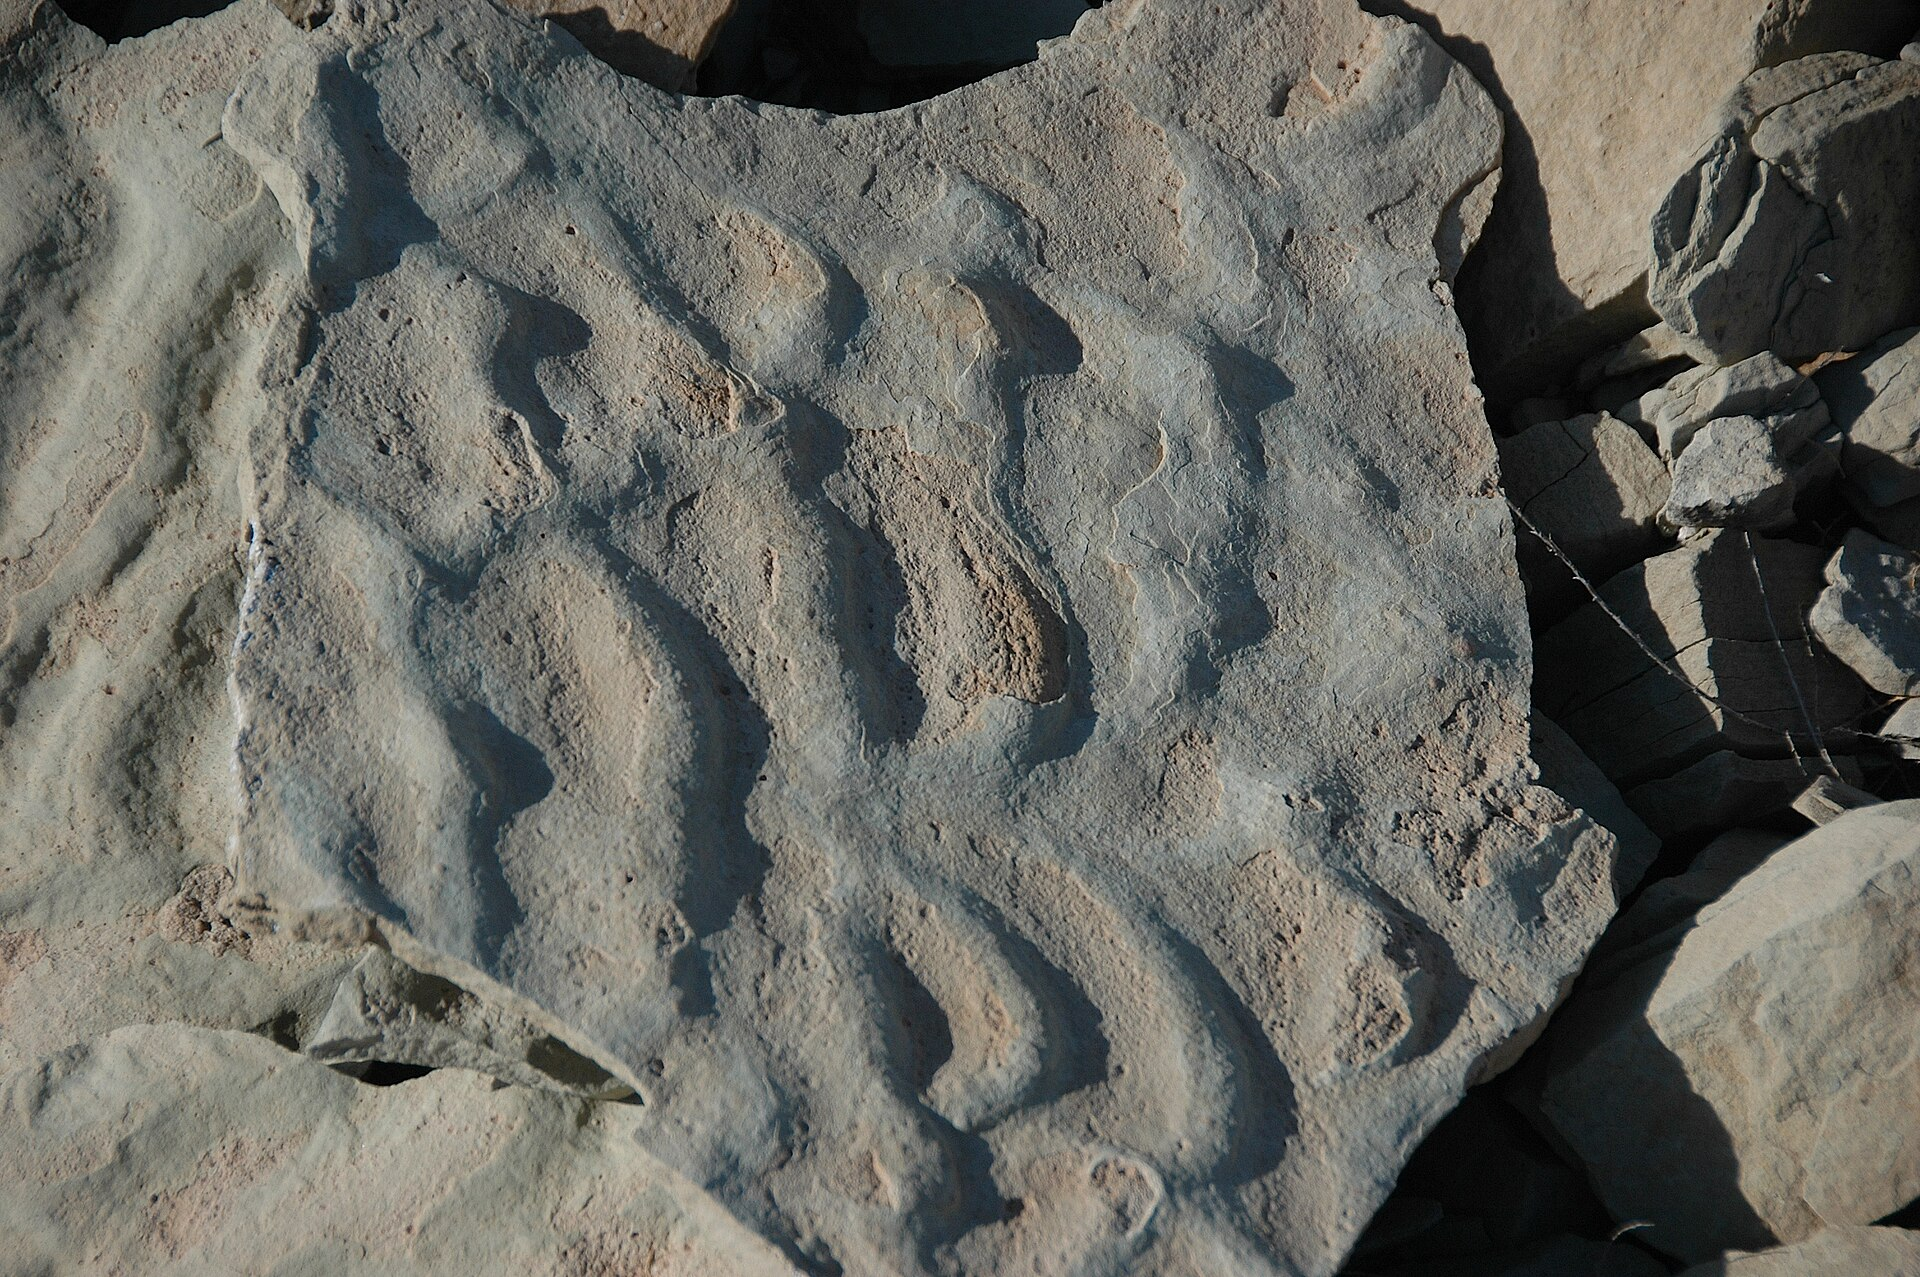
\includegraphics[width=0.56\linewidth]{images/book1/g7-ripple-marks.jpg}

{\small علامات تموج على لوح من الحجر الرملي في منتزه كابيتول ريف الوطني،
في يوتا (الولايات المتحدة): كان \omterm{def:g3:stones-pebbles-sand:sand}{الرمل} قد تموّج يومًا بفعل ماء متحرك، مثل
\omterm{def:g3:stones-pebbles-sand:sand}{رمل} شاطئ أو قاع جدول اليوم. الصورة: جيمس سانت~جون (CC BY 2.0، عبر
ويكيميديا كومنز).}
% ledger: commons:ripples, nps:ripple-marks
\label{fig:g7:sediments-and-fossils:ripples}
\end{omfigure}

\begin{example}[قمة الغراند كانيون]\label{ex:g7:sediments-and-fossils:kaibab}
حجر كايباب الجيري، الطبقة العليا في الغراند كانيون، مليء بأصداف عضديات
الأرجل وبقطع سيقان زنبقيات \omterm{def:g2:water-on-earth:ocean}{البحر}، وكلاهما من حيوانات \omterm{def:g2:water-on-earth:ocean}{البحر}. فقد تكوَّن في
قاع \omterm{def:g2:water-on-earth:ocean}{بحر}. واليوم تقع الطبقة نفسها على \omterm{def:g4:world-physical-map:altitude}{ارتفاع} يبلغ نحو \qty{2700}{m}
(\num{9000}~قدم) فوق مستوى \omterm{def:g2:water-on-earth:ocean}{البحر}: فمنذ تكوّنها، ارتفعت المنطقة كلها.
% ledger: nps:grca-fossils, nps:grca-kaibab
\end{example}

يمكن رسم كومة من الطبقات على شكل \emph{عمود}: الطبقات مكدسة بالترتيب
الذي تكونت به، وسماكاتها بمقياس رسم، وأدلتها مدوَّنة على الجانب. وعمود
تلال فاردن، المنطقة المُتخيَّلة لتمارين هذه السلسلة، معروض أدناه.

\begin{omfigure}
\begin{tikzpicture}
  \begin{axis}[width=4.2cm, height=9.2cm, scale only axis=false, xmin=0, xmax=1, ymin=-60, ymax=485,
      axis x line=none, axis y line*=left, ytick={0,100,200,300,400},
      ylabel={الارتفاع بالأمتار فوق قاعدة الحجر الرملي}, label style={font=\footnotesize},
      tick label style={font=\scriptsize}, clip=false]
    \addplot[lith schist, draw=black!70, line width=0.3pt] table {figdata/out/grade-7-varden_column-unit-older.dat};
    \addplot[lith sandstone, draw=black!70, line width=0.3pt] table {figdata/out/grade-7-varden_column-unit-sandstone.dat};
    \addplot[lith limestone, draw=black!70, line width=0.3pt] table {figdata/out/grade-7-varden_column-unit-limestone.dat};
    \addplot[lith shale, draw=black!70, line width=0.3pt] table {figdata/out/grade-7-varden_column-unit-shale.dat};
    \addplot[om lith={white}{om limestone}, draw=black!70, line width=0.3pt] table {figdata/out/grade-7-varden_column-unit-chalk.dat};
    \node[anchor=west, align=left, font=\footnotesize] at (axis cs:1.12,450) {\foreignlanguage{arabic}{\textbf{الطباشير}: تآكل سطحه}\\\foreignlanguage{arabic}{ولم تُرسم إلا قاعدته}};
    \node[anchor=west, align=left, font=\footnotesize] at (axis cs:1.12,350) {\foreignlanguage{arabic}{\textbf{السجّيل}، \babelsublr{\qty{100}{m}}: حبيبات دقيقة جدًا؛}\\\foreignlanguage{arabic}{أمونيت}};
    \node[anchor=west, align=left, font=\footnotesize] at (axis cs:1.12,210) {\foreignlanguage{arabic}{\textbf{الحجر الجيري}، \babelsublr{\qty{180}{m}}:}\\\foreignlanguage{arabic}{مرجان وأصداف}};
    \node[anchor=west, align=left, font=\footnotesize] at (axis cs:1.12,60) {\foreignlanguage{arabic}{\textbf{الحجر الرملي}، \babelsublr{\qty{120}{m}}:}\\\foreignlanguage{arabic}{علامات تموج، آثار أقدام}};
    \node[anchor=west, align=left, font=\footnotesize] at (axis cs:1.12,-30) {\foreignlanguage{arabic}{صخور أقدم من الشست والغرانيت}\\\foreignlanguage{arabic}{تآكلت حتى استوت قبل مجيء الحجر الرملي}};
  \end{axis}
\end{tikzpicture}

\medskip
{\small عمود تلال فاردن، المنطقة المُتخيَّلة في هذه السلسلة: الطبقات
بالترتيب الذي تكونت به، أولاها في الأسفل، وسماكاتها بمقياس رسم. \omterm{def:g7:sediments-and-fossils:fossil}{والأحافير}
والعلامات المدوَّنة على الجانب معطيات تمارين.}
% ledger: (invented region: figdata/shared/region.py, drawn by figdata/grade-7/varden_column.py)
\label{fig:g7:sediments-and-fossils:column}
\end{omfigure}

\begin{omfigure}
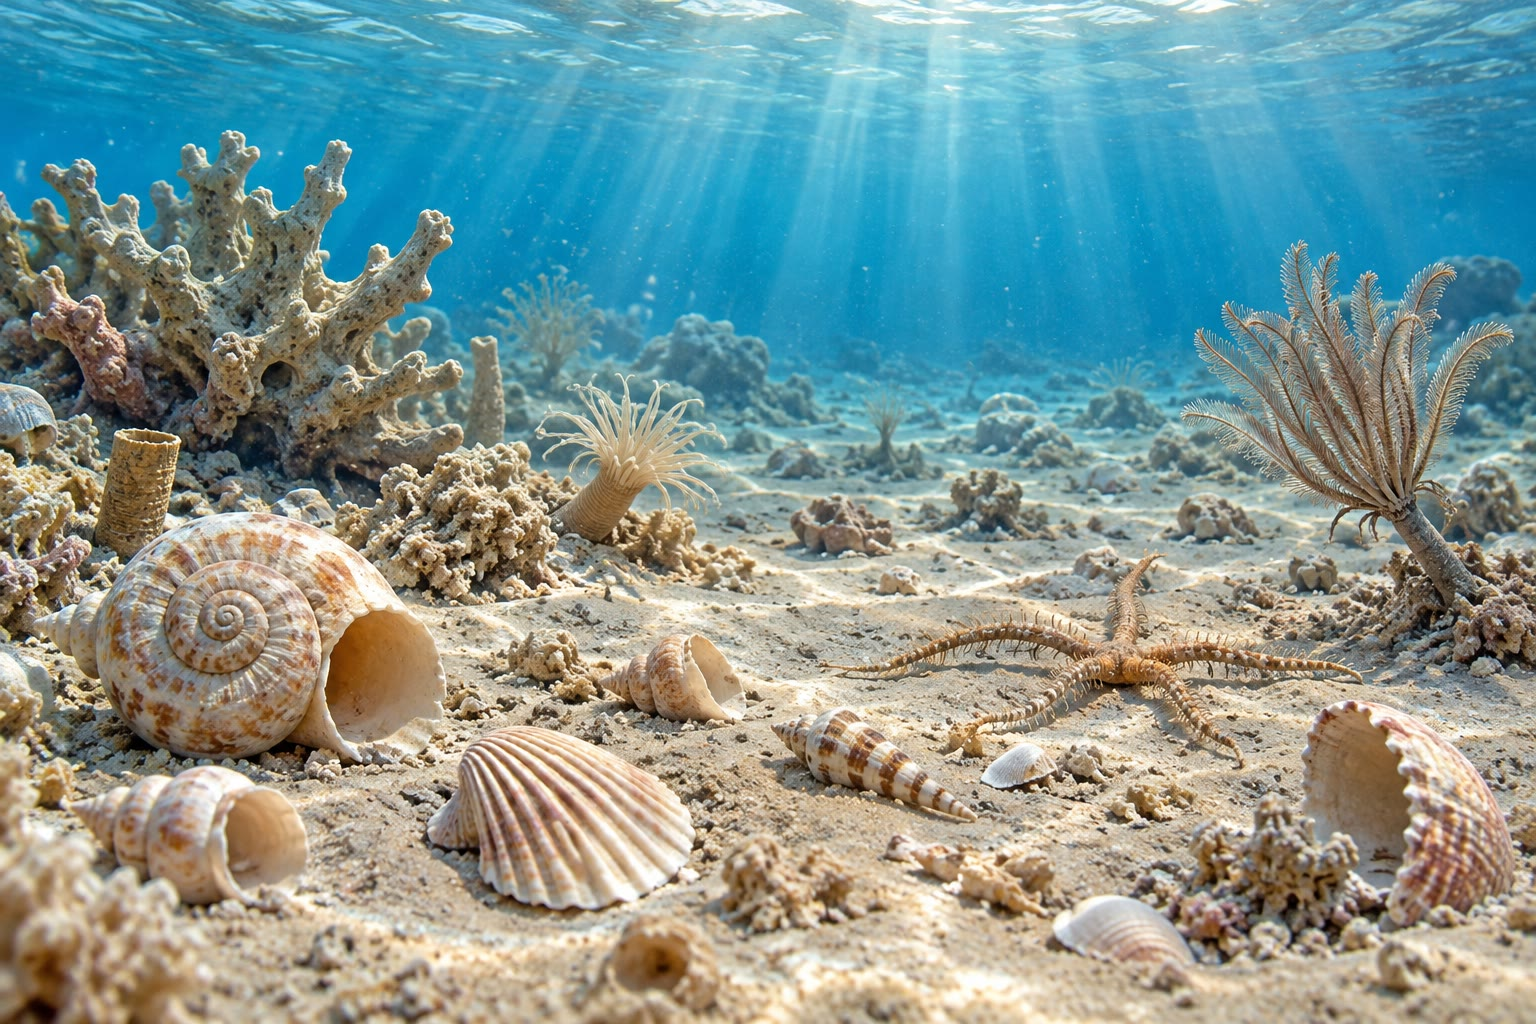
\includegraphics[width=0.6\linewidth]{images/book1/ai/g7-shallow-sea.jpg}

{\small قاع \omterm{def:g2:water-on-earth:ocean}{بحر} دافئ ضحل من زمن بعيد، كما قد يكون بدا بينما كانت الأصداف
وقطع المرجان تترسب لتصير حجرًا جيريًا في المستقبل (رسم توضيحي مولَّد
بالذكاء الاصطناعي لمشهد عام).}
\label{fig:g7:sediments-and-fossils:shallow-sea}
\end{omfigure}

\begin{remark}[انظر، وصوّر، واتركها]\label{rem:g7:sediments-and-fossils:leave}
في أماكن محمية كثيرة، يُمنع أخذ \omterm{def:g7:sediments-and-fossils:fossil}{الأحافير}: ففي الغراند كانيون مثلًا، يحظر
القانون حفر أي \omterm{def:g7:sediments-and-fossils:fossil}{أحفورة} أو تحريكها أو أخذها. والزائر الذي يجد واحدة
يصوّرها أو يرسمها، ويتركها في مكانها ليراها الآخرون ويدرسها العلماء،
ويخبر أحد الحراس.
\end{remark}
% ledger: nps:grca-fossils

\begin{inthefield}[رواسب تترسب اليوم]
على شاطئ، أو حافة \omterm{def:g1:landscapes-around-us:water}{بحيرة}، أو ضفة جدول، ومع شخص بالغ، انظر إلى \omterm{def:g3:stones-pebbles-sand:sand}{الرمل} تحت
الماء الضحل: فالماء المتحرك يشكّله تموجات، مثل تلك المحفوظة في الحجر
الرملي القديم. اترك أثر قدم في \omterm{def:g3:stones-pebbles-sand:sand}{الرمل} المبلل قرب حافة الماء وراقب ما تفعله
به الأمواج التالية. وبعد يوم ماطر، انظر إلى بركة صغيرة جفّت: كثيرًا ما
تغطي الرملَ في قاعها قشرةٌ رقيقة من \omterm{def:g3:stones-pebbles-sand:sand}{الوحل} الدقيق --- فأدق الحبيبات
ترسبت أخيرًا، حين كان الماء ساكنًا. ارسم ما تراه، ودوّن أين ومتى.
\end{inthefield}
% ledger: nps:ripple-marks, ucmp:footprints, usgs:strata

\section{تمارين}

\begin{exercise}[$\star$]\label{exo:g7:sediments-and-fossils:1}
صِل كل كلمة بمعناها: \omterm{def:g7:sediments-and-fossils:sediment}{الرواسب}؛ \omterm{def:g7:sediments-and-fossils:layer}{الطبقة الصخرية}؛ \omterm{def:g7:sediments-and-fossils:fossil}{الأحفورة}؛ \omterm{def:g7:sediments-and-fossils:fossil}{القالب}؛
\omterm{def:g7:sediments-and-fossils:fossil}{المصبوبة}؛ \omterm{def:g7:sediments-and-fossils:fossil}{الأحفورة الأثرية}. (أ) تجويف يبقى في \omterm{def:g3:stones-pebbles-sand:rock}{صخر} حيث ذابت صدفة. (ب) أثر
قدم أو جحر محفوظ في \omterm{def:g3:stones-pebbles-sand:rock}{صخر}. (ج) مواد مفككة يضعها الماء أو الريح أو الجليد.
(د) نسخة حجرية تتكون حين يمتلئ تجويف \omterm{def:g6:rocks-and-minerals:mineral}{بالمعادن}. (ه) صفيحة من \omterm{def:g7:sediments-and-fossils:sediment}{الرواسب}
وُضعت في وقت واحد. (و) بقايا كائن حي من زمن بعيد أو أثره، محفوظة في \omterm{def:g3:stones-pebbles-sand:rock}{صخر}.
\end{exercise}

\begin{exercise}[$\star$]\label{exo:g7:sediments-and-fossils:2}
رتّب هذه المراحل، لتحكي كيف تصير صدفة \omterm{def:g7:sediments-and-fossils:fossil}{أحفورة} على السطح: (أ) تبري \omterm{def:g5:water-shapes-the-land:erosion}{التعرية}
الطبقات التي فوقها؛ (ب) يموت الحيوان في قاع \omterm{def:g2:water-on-earth:ocean}{البحر}؛ (ج) تتراكم طبقات
جديدة وتتحول الصدفة إلى حجر؛ (د) يغطي \omterm{def:g3:stones-pebbles-sand:sand}{الوحل} الصدفة بسرعة.
\end{exercise}

\begin{exercise}[$\star$]\label{exo:g7:sediments-and-fossils:3}
استعمل جدول الأدلة. أين تكونت كل طبقة؟ (أ) حجر جيري مليء بالمرجان. (ب)
حجر رملي يُظهر سطحه علامات تموج. (ج) طبقة داكنة من الفحم. (د) سجّيل فيه
طبعات أوراق نبات وجناح يعسوب.
\end{exercise}

\begin{exercise}[$\star$]\label{exo:g7:sediments-and-fossils:4}
صواب أم خطأ؟ صحّح العبارات الخاطئة. (أ) كل حيوان يموت يصير \omterm{def:g7:sediments-and-fossils:fossil}{أحفورة} يومًا
ما. (ب) يمكن أن يكون أثر القدم \omterm{def:g7:sediments-and-fossils:fossil}{أحفورة}. (ج) حين يتباطأ ماء موحل، يترسب
\omterm{def:g3:stones-pebbles-sand:sand}{الوحل} الدقيق أولًا. (د) توضع \omterm{def:g7:sediments-and-fossils:sediment}{الرواسب} مستوية.
\end{exercise}

\begin{exercise}[$\star\star$]\label{exo:g7:sediments-and-fossils:5}
استعمل عمود تلال فاردن. (أ) أعطِ سماكة الحجر الرملي والحجر الجيري
والسجّيل. (ب) ما سماكتها الكلية؟ (ج) ما النسبة المئوية للحجر الجيري من
هذا المجموع؟ قرّب إلى أقرب عدد صحيح. (د) لماذا لا يعطي العمود أي سماكة
للطباشير؟
\end{exercise}

\begin{exercise}[$\star\star$]\label{exo:g7:sediments-and-fossils:6}
ترجّ تلميذة وعاءً فيه ماء \omterm{def:g3:stones-pebbles-sand:pebble}{وحصباء} \omterm{def:g3:stones-pebbles-sand:sand}{ورمل} \omterm{def:g3:stones-pebbles-sand:sand}{ووحل}، ثم تتركه يترسب. (أ) ارسم
الوعاء في اليوم التالي، وسمِّ الطبقات. (ب) لماذا يبقى الماء عكرًا بعد
ساعة؟ (ج) تضيف \omterm{def:g3:stones-pebbles-sand:sand}{الرمل} \omterm{def:g3:stones-pebbles-sand:sand}{والوحل} من جديد وتتركه يترسب. ماذا ترى في القاع
الآن؟ (د) أي طبقات الوعاء تكونت أولًا؟
\end{exercise}

\begin{exercise}[$\star\star$]\label{exo:g7:sediments-and-fossils:7}
أي هذه لديه أفضل فرصة ليصير \omterm{def:g7:sediments-and-fossils:fossil}{أحفورة}، وأيها أقل فرصة؟ اشرح. (أ) قنديل \omterm{def:g2:water-on-earth:ocean}{بحر}
قذفته الأمواج على شاطئ صخري. (ب) صدفة حلزون مدفونة في \omterm{def:g3:stones-pebbles-sand:sand}{وحل} \omterm{def:g1:landscapes-around-us:water}{بحيرة} هادئة.
(ج) عظم ملقى سنوات على \omterm{def:g1:landscapes-around-us:landform}{سهل} جاف. (د) صدفة محار غطاها \omterm{def:g3:stones-pebbles-sand:sand}{الرمل} في \omterm{def:g5:water-shapes-the-land:flood}{فيضان} \omterm{def:g1:landscapes-around-us:water}{نهر}.
\end{exercise}

\begin{exercise}[$\star\star$]\label{exo:g7:sediments-and-fossils:8}
دُفنت صدفة في \omterm{def:g3:stones-pebbles-sand:sand}{رمل} صار حجرًا رمليًا. ويذيب الماء المتسرب عبر \omterm{def:g3:stones-pebbles-sand:rock}{الصخر} الصدفة
تمامًا. (أ) ماذا يبقى في \omterm{def:g3:stones-pebbles-sand:rock}{الصخر}؟ (ب) لاحقًا، تملأ \omterm{def:g6:rocks-and-minerals:mineral}{معادن} هذا التجويف. ماذا
يتكون؟ (ج) هل الصدفة نفسها لا تزال هناك؟ (د) لماذا توجد \omterm{def:g7:sediments-and-fossils:fossil}{القوالب} \omterm{def:g7:sediments-and-fossils:fossil}{والمصبوبات}
في الحجر الرملي أكثر مما توجد في السجّيل؟ (فكّر في سهولة مرور الماء بين
الحبيبات.)
\end{exercise}

\begin{exercise}[$\star\star$]\label{exo:g7:sediments-and-fossils:9}
يبلغ عمق الغراند كانيون \qty{1.6}{km} في المتوسط. (أ) اكتب هذا العمق
بالأمتار. (ب) افترض أن جدران \omterm{def:g1:landscapes-around-us:landform}{الوادي} مكوَّنة من طبقات سماكة كل منها
\qty{80}{m}: كم طبقة تتسع من الحافة إلى القاع؟ (ج) طبقة سماكتها
\qty{160}{m} تمثل أي نسبة مئوية من العمق؟
\end{exercise}

\begin{exercise}[$\star\star$]\label{exo:g7:sediments-and-fossils:10}
توجد آثار أقدام ديناصورات في حجر رملي. (أ) هل كانت الديناصورات تمشي على
\omterm{def:g3:stones-pebbles-sand:rock}{صخر} صلب؟ اشرح. (ب) لماذا تختفي معظم آثار الأقدام المتروكة على شاطئ موحل؟
(ج) ماذا كان يجب أن يحدث بعد مرور الديناصورات بقليل لكي تُحفظ الآثار؟
(د) هل أثر القدم \omterm{def:g7:sediments-and-fossils:fossil}{أحفورة} جسمية أم \omterm{def:g7:sediments-and-fossils:fossil}{أحفورة أثرية}؟
\end{exercise}

\begin{exercise}[$\star\star\star$]\label{exo:g7:sediments-and-fossils:11}
في \omterm{def:g1:landscapes-around-us:water}{بحيرة}، يترك كل \omterm{def:g5:water-shapes-the-land:flood}{فيضان} طبقة من \omterm{def:g3:stones-pebbles-sand:sand}{الرمل} سماكتها نحو \qty{2}{cm}، وتترك
الأسابيع الهادئة التي تليه طبقة من \omterm{def:g3:stones-pebbles-sand:sand}{الوحل} سماكتها نحو \qty{5}{mm}
(معطيات تمرين). (أ) ما سماكة زوج واحد من الطبقات، بالمليمترات؟ (ب) جزرة
حفر أُخذت من قاع \omterm{def:g1:landscapes-around-us:water}{البحيرة} طولها \qty{1}{m}، ولا تتكون إلا من أزواج كهذه.
كم فيضانًا تسجل؟ (ج) قرب \omterm{def:g5:water-shapes-the-land:source-mouth}{مصب} \omterm{def:g1:landscapes-around-us:water}{النهر} تكون طبقات \omterm{def:g3:stones-pebbles-sand:sand}{الرمل} أسمك، وبعيدًا عنه
تكون أرق. اشرح لماذا. (د) لماذا يكون \omterm{def:g3:stones-pebbles-sand:sand}{الوحل} أكثر من \omterm{def:g3:stones-pebbles-sand:sand}{الرمل} بعيدًا عن
\omterm{def:g5:water-shapes-the-land:source-mouth}{المصب}؟
\end{exercise}

\begin{exercise}[$\star\star\star$]\label{exo:g7:sediments-and-fossils:12}
\omterm{def:g7:sediments-and-fossils:fossil}{الأحافير} التي توجد في \omterm{def:g3:stones-pebbles-sand:rock}{الصخور} هي في معظمها أصداف وبقايا دقيقة؛ أما \omterm{def:g7:sediments-and-fossils:fossil}{أحافير}
الحيوانات الطرية فنادرة، وليست الديناصورات إلا جزءًا صغيرًا جدًا من كل
\omterm{def:g7:sediments-and-fossils:fossil}{الأحافير}. (أ) اشرح لماذا الأصداف شائعة إلى هذا الحد. (ب) اشرح لماذا
الحيوانات الطرية نادرة. (ج) يريد عالم أن يعرف كل الحيوانات التي عاشت في
\omterm{def:g2:water-on-earth:ocean}{بحر} قديم. هل تستطيع \omterm{def:g7:sediments-and-fossils:fossil}{الأحافير} أن تعطي القائمة الكاملة؟ اشرح.
\end{exercise}

\section{مسألة: عمود تلال فاردن}

\begin{problem}[{مسألة نهاية الأسبوع --- تُقرأ طبقات تلال فاردن واحدة
بعد أخرى، وتخبر أحافيرها أين تكونت، ويُحسب الزمن اللازم لتراكم الحجر
الجيري}]
\label{pb:g7:sediments-and-fossils:1}
% ledger: (invented region: figdata/shared/region.py; rates are exercise data, figdata/grade-7/varden_column.py part rates)
استعمل عمود تلال فاردن في هذا الفصل. يُظهر حجره الرملي علامات تموج وآثار
أقدام؛ ويحوي حجره الجيري مرجانًا وأصدافًا؛ ويتكون سجّيله من حبيبات دقيقة
جدًا، وفيه أمونيت؛ أما الطباشير في الأعلى فقد تآكل جزء منه.

\medskip
\noindent\textbf{الجزء الأول --- قراءة الطبقات.}\par\nopagebreak
\begin{enumerate}[beginpenalty=10000]
  \item اذكر الطبقات الأربع، من أولاها ترسبًا إلى آخرها.
  \item أعطِ سماكة الحجر الرملي والحجر الجيري والسجّيل، ومجموعها.
  \item ما النسبة المئوية للحجر الجيري من هذا المجموع؟
  \item لماذا لا يستطيع أحد أن يقول كم كانت سماكة الطباشير حين تكوّن؟
\end{enumerate}

\medskip
\noindent\textbf{الجزء الثاني --- الأحافير التي فيها.}\par\nopagebreak
\begin{enumerate}[resume, beginpenalty=10000]
  \item أين تكوّن الحجر الرملي؟ أعطِ دليلين.
  \item أين تكوّن الحجر الجيري؟ أعطِ الدليل.
  \item يتكون السجّيل من حبيبات دقيقة جدًا. هل كان الماء هادئًا أم متحركًا
        حين ترسب؟ اشرح.
  \item احكِ قصة المكان في ثلاث جمل، من الحجر الرملي إلى السجّيل.
\end{enumerate}

\medskip
\noindent\textbf{الجزء الثالث --- كم استغرق ذلك.}\par\nopagebreak
\begin{enumerate}[resume, beginpenalty=10000]
  \item اكتب سماكة الحجر الجيري بالسنتيمترات.
  \item افترض أن الحجر الرملي تراكم بمعدل \qty{1}{cm} كل 20 سنة. فكم
        سنة استغرقت سماكته البالغة \qty{120}{m}؟
  \item افترض أن الحجر الجيري تراكم بمعدل \qty{1}{cm} كل 100 سنة.
        فكم سنة استغرق \qty{1}{m} من الحجر الجيري؟
  \item كم سنة استغرقت \qty{180}{m} من الحجر الجيري؟ وكم مرة يزيد ذلك
        على زمن الحجر الرملي؟
\end{enumerate}
\end{problem}
